\documentclass[10pt,twocolumn]{article}
\usepackage{titling}
\usepackage{hyperref}

\usepackage{tikz}
\usetikzlibrary{calc, arrows}

\usepackage{float}
\floatstyle{boxed}
\restylefloat{figure}

\usepackage{adjustbox}

\newcommand{\subtitle}[1]{%
  \posttitle{%
    \par\end{center}
    \begin{center}\large#1\end{center}
    \vskip0.5em}%
}

\title{Poetwriter: A Constraint-Based Novel Text Generator}
\subtitle{
	CS 221 Final Project\\
	Stanford University
	}
\author{
	Mathieu Rolfo\\
	\href{mailto:rolfom01@stanford.edu}{rolfom01@stanford.edu}
  \and
  	Shalom Rottman-Yang\\
	\href{mailto:jaronry@stanford.edu}{jaronry@stanford.edu}
  \and
  	Nathan James Tindall\\
	\href{mailto:ntindall@stanford.edu}{ntindall@stanford.edu}
}
\date{12 December 2014}

\begin{document}

\maketitle

\section{Introduction}
Poetry is one of the most expressive ways to use verbal language. It is notoriously difficult for humans to produce, and the study of what delineates good and bad poetry is a vibrant academic field. Poetry is unique in that both content and form contribute to its aesthetic value. The interlinking of these aspects creates difficult problems for poetry generation, requiring careful algorithmic design and natural language processing to solve. In the remainder of this report, we will define poetry as text with semantic coherence that meets specified formal constraints. The ability to produce quality poetry represents a thought-provoking intersection between human and computational intelligence.

\section{Related Work}
A sizable amount of research has been performed on text generation. Some existing approaches to creative computation have generated poetry by performing word substitution on a set of poems that serve as the training data for the model. Under this view, producing novel syntactic structure is not a sub-problem of producing valuable poetry. Instead, researchers have found success by invoking a semantic network in order to perform intelligent substitution of noun and verb phrases of existing poetry, in an attempt to generate novel content. For example, a Shakespearian soliloquy might be changed from being an elaboration on the beauty of roses to a discourse on the flowing nature of water, with the following substitutions: pink $\rightarrow$ flowing, flower $\rightarrow$ water, falling $\rightarrow$ trickling. However, these existing models have usually not imposed rhyming or syllabic constraints on the poems. Existing work on matching predefined rhyme and syllabic schemes, as well as utilizing unusual corpora (e.g. rap lyrics, legal documents) is very limited.

\section{Task Definition}
Our task for this project was to design a framework for poetry generation that allows a human to give a corpus as input and specify formal constraints, and have our intelligent creation generate novel, semantically meaningful poetry meeting those constraints. Our algorithm has special optimizations for the corpora of rap artists in an attempt to generate rap-styled poetry; however, the general case of the problem is one of poetic generation. In this project, our constraints are on the syllable counts of lines and the rhyming patterns between lines. 

\section{Approach}
As stated above, we chose to break the problem into two subproblems: the production of content and the resolution of formal constraints inherent to poetry. For the content subproblem, we chose to use a n-gram model, and for the resolution subproblem, we selected a constrained search paradigm. 

Our n-gram model forms the basis of the language model for generation. n-gram models are common bases for language models, relying on the properties of syntax that can be predicted by probabilistic inference, rather than by application of formal rules. n-gram models have been able to achieve robust results in other research, including text reconstruction. Although other formal systems could be used, such as the application of syntax generators in order to generate new sentences, we believed that the n-gram model served our purposes better because it is able to directly capture the probabilistic essence of corpora. Additionally, the model is flexible: it is not inherently clear whether higher n results in higher quality poetry, as poetry may not benefit from a richer context that models trained on higher n values provide. 

The formal constraints of poetry can be viewed as a natural application of a constraint satisfaction problem. Considering the fact that all poetry is comprised of lines, we can view the constraints on poetry as a combination of intra-line constraints and inter-line constraints. Intra-line constraints include the number of syllables allowed on each line, the meter of the rhyme, and any additional features of poetry and rhetoric that are independent from the state of other lines in the poem, such as internal rhyme and metaphor. Inter-line constraints consist of rhyming pairs.

Our algorithm for resolution is an instantiation of depth first search with arm's length backtracking. Because our rhyme constraints only are considered on the final word of a line, using depth first search is more efficient than using backtracking search for constraint checking and allows for rapid end-line state evaluation.

\section{Baseline}
Our baseline is a probabilistic n-gram model that produces strings after being trained on an corpus. The baseline lacks rhyming constraints and semantic checking; however, it is able to produce rhetoric that uses the corpus' lexicon, relying on the n-gram model to produce semantically consistent prose. As a simplifying assumption, the baseline assumes that a line of poetry has eight words, as a stand-in for syllabic constraints. The first word of each line is based on the n-gram value of the last n words on the previous line. Additionally, the baseline assumes that poetry has 15 lines and a standard form (same number of syllables per line, etc.). See appendix for output examples.

Our analysis of the output generated by the n-gram model is that while the unigram model produces phrases that are grammatically and semantically inconsistent, the trigram model frequently just reproduces lines from the corpus verbatim. In the scope of the baseline, this may be a function of the size of the corpus alone, such that a trigram model may succeed at generating novel output once rhyming and syllabic constraints are imposed; however, it is also an indicator that unigram features alone may not be sufficient in order to produce novel output, given the size of our corpus. This may prompt us to add additional syntactic feature indicators as we proceed in our developmental process.

\section{Oracle}
The oracle for this problem is asking a human to write poetry, which we define as text satisfying constraints placed on syllable count and rhyme pattern. This is something that humans can do with high accuracy, creativity, and expression. Humans are very good at generating poetry that is consistent with poetic paradigms. For a given form (e.g. the sonnet), humans will be able to generate satisfactory output with almost 100\% accuracy if constraints on meaning or poetic quality are not in place. 

\section{Advanced Method}
Our advanced method performs depth-first-search over the n-gram model in order to satisfy the constraints defined at runtime. We define this search problem as follows:
\begin{enumerate}
	\item \verb!startState!: current state of poem, current state of n-gram model (seed)
	\item \verb!action!: adding a valid word to the poem and updating the n-gram seed
	\item \verb!isGoal(state)!: if constraints of poem have been satisfied
	\item \verb!succAndCost(state)!: returns a list of valid (word, (new poem, new seed), word frequency) tuples, where (new poem, new seed) is a successor pair for (poem, seed) that satisfies the constraints of the model (only valid actions taken). 
	\end{enumerate}
\begin{figure}
\caption{Search through corpus model model with \emph{n} $= 1$}
\centering
\adjustbox{max width = \linewidth}{
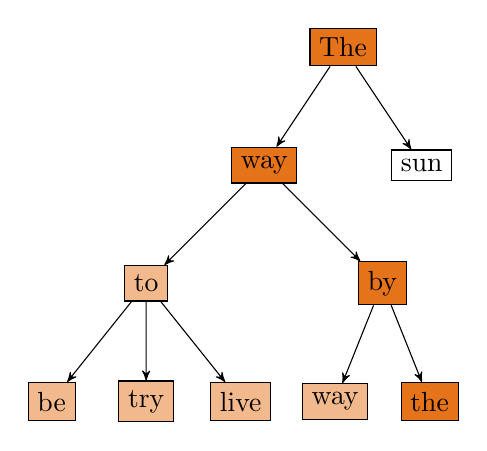
\begin{tikzpicture}[->,>=stealth',every node/.style={circle,draw},level 1/.style={sibling distance=20mm},level 2/.style={sibling distance=30mm},level 3/.style={sibling distance=12mm},
%scale=0.7, transform shape
]
\node [shape=rectangle,fill = orange!90!blue](nA){The}
   child { node[shape=rectangle,fill = orange!90!blue] (nB) {way}
              child { node[shape=rectangle,fill = orange!90!blue!50] (nD) {to}
                         child { node[shape=rectangle,fill = orange!90!blue!50] (nH) {be} }
                         	child { node[shape=rectangle,fill = orange!90!blue!50] (nI)  {try} }
                         child { node[shape=rectangle, fill = orange!90!blue!50] (nJ) {live} }
                       }
              child {  node [shape=rectangle,fill = orange!90!blue] (nE) {by}
                         child { node [shape=rectangle,fill = orange!90!blue!50] (nK) {way} }
                         child { node [shape=rectangle,fill = orange!90!blue] (nL) {the} }
                       }
            }
   child { node (nC) [shape=rectangle,] {sun}
           };

\end{tikzpicture}
}
\end{figure}

\begin{figure}
\caption{Search through corpus model with \emph{n} $= 2$}
\centering
\adjustbox{max width =\linewidth}{
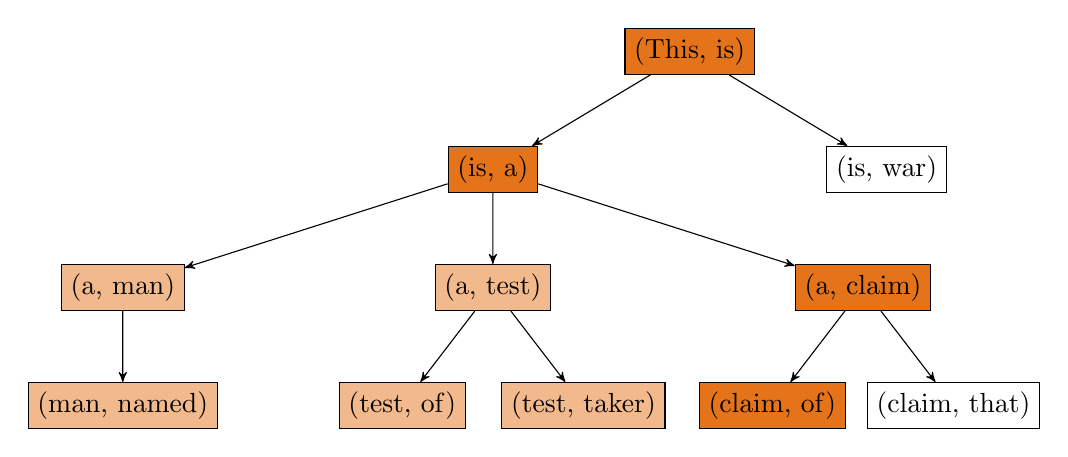
\begin{tikzpicture}[->,>=stealth',every node/.style={circle,draw},level 1/.style={sibling distance=50mm},level 2/.style={sibling distance=47mm},level 3/.style={sibling distance=23mm},
%scale=0.7, transform shape
]
\node [shape=rectangle,fill = orange!90!blue](nA){(This, is)}
   child { node[shape=rectangle,fill = orange!90!blue] (nB) {(is, a)}
              child { node[shape=rectangle,fill = orange!90!blue!50] (nD) {(a, man)}
                         child { node[shape=rectangle,fill = orange!90!blue!50] (nH) {(man, named)} }
                       }
              child { node[shape=rectangle,fill = orange!90!blue!50] (nM) {(a, test)}
                         child { node[shape=rectangle,fill = orange!90!blue!50] (nN) {(test, of)} }
                         child { node[shape=rectangle,fill = orange!90!blue!50] (nO) {(test, taker)} }
                       }
              child {  node [shape=rectangle,fill = orange!90!blue] (nE) {(a, claim)}
                         child { node [shape=rectangle,fill = orange!90!blue] (nK) {(claim, of)} }
                         child { node [shape=rectangle] (nL) {(claim, that)} }
                       }
            }
   child { node (nC) [shape=rectangle,] {(is, war)}
           };

\end{tikzpicture}
}
\end{figure}

Principal among challenges we faced during development were formalizing the rhyme and syllabic constraints, specifically: 1. how to incorporate these constraints into the model in order to direct the depth first search 2. how to evaluate the number of syllables in a word, 3. how to determine if two words rhyme, and 4. limitations of corpora. Important for the success of 2-4 was the utilization of Moby Python IPA Dictionary. 
\begin{enumerate}
\item is solved by a propagator-receiver framework in which end-line constraints are imposed in the forwards direction after a rhyme-propagating rhyme is completed. For example, if lines 0 and 1 are designated to rhyme, then after the search has completed line 0, the rhyming constraint is propagated forwards onto line 1 (the receiver). This facilitates forward motion but also allows the algorithm to backtrack by arm's length when it gets stuck.

\item For each element of the IPA dictionary, the number of IPA vowels was counted and used as an estimate for the number of syllables in each word of the dictionary. Most IPA transcriptions of words lacked digraphs (successive vowels), resulting in a fairly accurate syllable estimate. If a word in the corpus is not in the dictionary, an alternative estimate based upon word length is used. 

\item In our algorithm, the suffix for an entry in the IPA dictionary is defined as the substring starting at the last vowel in the word. Two words rhyme if their suffixes match. If one of the words is not in the IPA dictionary, a similar estimate is used based solely upon their standard alphabet spelling. Though rhyme detection is crucial to the success of the model, its development is auxiliary to the scope of our project as a whole. Thus, after experimenting with a number of syllable-estimation techniques, we found that this estimate was accurate for the majority of words output through generation.

\item Unfortunately, the model does not always produce results, and this is primarily a result of corpora that are small enough that the n-gram generator cannot find rhyming pairs. In order to solve this problem, we had ideas of being able to relax the way that words are selected in order to choose rhyming nouns outside of the corpus, though this would detract from the character of the corpora. 
\end{enumerate}
Secondly among challenges addressed were algorithmic changes in order to make the output of the poem more semantically meaningful. In an attempt to increase the semantic quality of poems generated, we took four approaches: 1. grouping pairs of lines as semantic sentences, 2. tracking beginning words in the n-gram model in order to better approximate proper language  3. cleaning the corpora in order to remove extraneous words, and 4. imposing part of speech constraints on the format of the poems.
\begin{enumerate}
\item Initially, our n-gram model was trained on the entire corpus text unbroken. This led to the generator producing a continuous stream of text throughout the poem, which hindered semantic quality. To fix this, we added in the ability to reseed the poem anew after a given number of lines. Thus, the text in the poem was broken into smaller parts, allowing the poem to be composed of semantic sentences - streams of n-gram generated text from separate seeds. This paved the way for other approaches to enforce meaning contained within distinct sentences. The frequency of reseeding is specifiable at runtime. 

\item Even with the imposition of sentence structure on the poems, the meaning of the generated text was largely incomprehensible. A large reason for this was that the sentences would begin apparently in the middle of meaningful text, because the reseeding technique did not require the beginning of a sentence to represent the beginning of a phrase. To address this, special BEGIN words were incorporated into the corpus between lines. This served two purposes: the n-gram model would not remember following words for a seed if those words were part of a semantically separate sentence (we assumed that each line of the corpus was a separate sentence); and upon generation, the model could require that the starting seed for a new sentence be chosen from known sentence initiators.

\item Certain corpora contain formatting or organizational phrases, e.g. verse and hook in song lyrics. Therefore, we added the possibility to tailor the n-gram model to different corpus sources by trimming these extraneous phrases from the corpus before analyzing it.
\item
\end{enumerate}




\section{Data \& Experiments}

\section {Analysis}

\section{Conclusion}

\section{References}


\end{document}